\documentclass[border=0.1cm, 12pt]{standalone}
\usepackage[utf8]{inputenc}

\usepackage{tikz}
\usepackage{amsfonts}
\usepackage{amsmath,amssymb}
\usepackage{systeme,mathtools}
\usetikzlibrary{positioning,arrows.meta,quotes}
\usetikzlibrary{shapes,snakes}
\usetikzlibrary{bayesnet}
\tikzset{>=latex}

\begin{document}
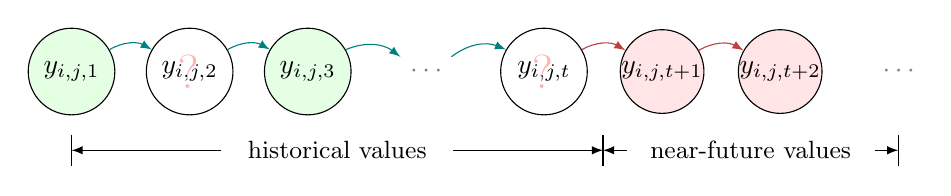
\begin{tikzpicture}
\node[circle,draw=black,fill=green!10,inner sep=0pt,minimum size=1.1cm] (obs1) at (0,0) {$y_{i,j,1}$};
\node[circle,draw=black,fill=white,inner sep=0pt,minimum size=1.1cm] (obs2) at (1.5,0) {$y_{i,j,2}$};
\node[circle,draw=black,fill=green!10,inner sep=0pt,minimum size=1.1cm] (obs3) at (3,0) {$y_{i,j,3}$};
\node[text width=0.4cm] (obs4) at (4.5,0) {\color{gray}{$\LARGE{\cdots}$}};
\node[circle,draw=black,fill=white,inner sep=0pt,minimum size=1.1cm] (obs5) at (6,0) {$y_{i,j,t}$};
\node[circle,draw=black,fill=red!10,inner sep=0pt,minimum size=0.8cm] (obs6) at (7.5,0) {$y_{i,j,t+1}$};
\node[circle,draw=black,fill=red!10,inner sep=0pt,minimum size=0.8cm] (obs7) at (9,0) {$y_{i,j,t+2}$};
\node[text width=0.4cm] (obs8) at (10.5,0) {\color{gray}{$\LARGE{\cdots}$}};
\path [draw,->,color=blue!50!green] (obs1) edge [bend left] node [right] {} (obs2);
\path [draw,->,color=blue!50!green] (obs2) edge [bend left] node [right] {} (obs3);
\path [draw,->,color=blue!50!green] (obs3) edge [bend left] node [right] {} (obs4);
\path [draw,->,color=blue!50!green] (obs4) edge [bend left] node [right] {} (obs5);
\path [draw,->,color=red!50!gray] (obs5) edge [bend left] node [right] {} (obs6);
\path [draw,->,color=red!50!gray] (obs6) edge [bend left] node [right] {} (obs7);
\node[text width=0.3cm] (unknown1) at (1.5,-0.0) {\LARGE\color{red!30}{?}};
\node[text width=0.3cm] (unknown1) at (6,-0.0) {\LARGE\color{red!30}{?}};

\draw[] (0,-0.8) -- (0,-1.2);
\draw[] (6.75,-0.8) -- (6.75,-1.2);
\draw[] (10.5,-0.8) -- (10.5,-1.2);
\node at (3.375,-1) {\small{historical values}};
\draw[arrows=->] (4.85,-1)--(6.75,-1);
\draw[arrows=<-] (0,-1)--(1.9,-1);
\node at (8.625,-1) {\small{near-future values}};
\draw[arrows=->] (10.2,-1)--(10.5,-1);
\draw[arrows=<-] (6.75,-1)--(7.05,-1);

\end{tikzpicture}
\end{document}
